% !TeX root = thesis.tex

\chapter{Literature study}\label{ch:literature-study}
In this chapter, we discuss existing research relevant to uncertainty in \gls{ai} models and how it maps to real-world scenarios.
First, we elaborate on what uncertainty is and the different ways it can sneak into \gls{ai} models.
Next, we discuss how this uncertainty can be quantified.
Finally, we explore existing methods to make \gls{ai} models uncertainty-aware and discuss how these concepts apply to a regression problem.

\section{Uncertainty in AI} \label{ch:literature-study_section:uncertainty-in-ai}
Many complex systems need to be modeled and understood.
These systems can be modeled using \gls{ai} models, which offer a way to grasp their complexity and operate them as efficiently and safely as possible.
However, like humans, these models are not perfect and can make mistakes.
When using standard, non-uncertainty-aware \gls{ai} models, these mistakes are not communicated to the user.
For example, when a \gls{cnn} is used to detect an object on a conveyor belt, it outputs the predicted class without indicating its certainty about the prediction.
If the object is only partially visible, the lighting is poor, or the object closely resembles another, the model might be highly uncertain but will still output a class as if it were confident.
All possible uncertainties regarding \glspl{dnn} can be categorized into two groups: aleatoric uncertainty and epistemic uncertainty~\cite{src:survey-uncertainty-dnn}~\cite{src:scalable-bayesian-deep-learning}.

\subsection{Aleatoric uncertainty}\label{ch:literature-study_section:uncertainty-in-ai_subsection:aleatoric-uncertainty}
Aleatoric uncertainty is a type of uncertainty that arises from noise inherent in the data.
Its nature is irreducible, meaning this uncertainty will remain present regardless of how much data is gathered.

\paragraph{Measurement errors}\label{ch:literature-study_section:uncertainty-in-ai_paragraph:measurement-errors}
When gathering data, mistakes can be made during the measuring process.
These often stem from limitations of the measurement devices or imprecise data labeling.
It is important to note that, if kept subtle, these mistakes can actually serve as a way to regularize a network.

As an example, we consider a regression problem where a model predicts the $x$ and $y$ coordinates for the center of an object.
The camera used for data capture might have a low resolution, and thus a lack of pixels which could cause an object to apear differently.
Furthermore, it could lead to inaccurate annotations; the center might be labeled as $(x_1, y_1)$ when it is actually $(x_1+\delta, y_1+\epsilon)$, with $\delta$ and $\epsilon$ representing small measurement errors.

\subsection{Epistemic uncertainty}\label{ch:literature-study_section:uncertainty-in-ai_subsection:epistemic-uncertainty}
Epistemic uncertainty originates from noise within the model or its training process.
This can stem from various causes, such as the model's architecture, the training procedure, or a lack of knowledge due to insufficient or irrelevant training data.
In theory, its nature is reducible, meaning that gathering better data or using a better suited model architecture can decrease this uncertainty.
However, doing so in practice carries a significant computational cost, making it not always feasible to eliminate this uncertainty.

\paragraph{Variability in real world situations} \label{ch:literature-study_section:uncertainty-in-ai_subsection:epistemic-uncertainty_paragraph:variability-in-real-world-situations}
The real world changes constantly, creating diverse settings where objects may behave or look differently.
Ideally, all potential situations should be sufficiently covered by the training set.
If not, the network trained on this data cannot guarantee accurate outputs for new real-world situations.
A distribution shift occurs when these real-world scenarios differ from the training data.
These shifts are highly challenging for a \gls{dnn} to process, causing its performance to fluctuate significantly.

Continuing with the regression problem of predicting an object's center.
When a \gls{dnn} is trained on a dataset featuring optimal lighting and no occlusions, no other objects covering the view, etc., it will perform well in that specific setting.
However, during actual inference, conditions might change unexpectedly, such as altered lighting, the appearance of new objects, etc.
Because the dataset lacks examples of these new conditions, the trained \gls{dnn} fails to adapt, leading to a drop in performance.

\paragraph{Architecture specification errors} \label{ch:literature-study_section:uncertainty-in-ai_subsection:epistemic-uncertainty_paragraph:architecture-specification-errors}
Network structures differ significantly, with each architecture having specific advantages and disadvantages regarding performance and prediction uncertainty.

Suppose a factory requires the previously discussed regression model to meet their needs.
Numerous model architectures are available, such as an \gls{mlp}, a \gls{cnn}, a U-net~\cite{src:u-net}, a \gls{gan}, or a YOLO network~\cite{src:yolo}, etc.
Each model has its own configuration of layers, connections, and activation functions.
Consequently, all these networks will have their own capabilities and thus uncertainty for a given task.

\paragraph{Training procedure errors} \label{ch:literature-study_section:uncertainty-in-ai_subsection:epistemic-uncertainty_paragraph:training-procedure-errors}
During model training, there are many decisions that need to be made.
These include selecting the learning rate, the number of epochs, the data batching strategy, the optimizer, the weight initialization, etc.
Each combination of these hyperparameters results in a different model with its own specific errors and uncertainty.

For instance, the dataset for object center regression can be split into different batch sizes, ordered in various ways, etc.
The chosen architecture can be trained using these diverse data handling methods, using different parameters to optimize it.
This again leads to varying models that perform better in certain areas but poorly in others.

\paragraph{Errors by unknown data} \label{ch:literature-study_section:uncertainty-in-ai_subsection:epistemic-uncertainty_paragraph:errors-by-unknown-data}
Once fully trained, the model may encounter entirely unprecedented situations during inference.
Although unexpected within the original problem scope, the model must process these situations, resulting in high uncertainty.

In the factory example, the model is trained for a specific environment and objective: detecting object centers in an industrial setting.
If an unexpected object, such as a bird, enters the camera's viewpoint, the model will be highly uncertain because it has never seen one before.
This occurs not because the environment was insufficiently tought to the model, but due to the completely unexpected nature of the bird being in the factory.

\subsection{Sources of uncertainty} \label{ch:literature-study_section:uncertainty-in-ai_subsection:sources-of-uncertainty}
In our specific problem of object localization for robotic arm grasping, both aleatoric and epistemic uncertainties are present.
We would like to tackle both!

First is the aleatoric uncertainty, inherent in the data, primarily caused by measurement errors.
While we will attempt to minimize these errors, they will inevitably remain present in the dataset.
However, as mentioned in \cref{ch:literature-study_section:uncertainty-in-ai_subsection:aleatoric-uncertainty}, these errors are not the primary concern; if kept subtle, they can act as a form of model regularization.

One of the sources of aleatoric uncertainty are the errors introduced during the data collection and annotation process.
More concretely, when indicating the center of an object in the image, the annotator will not be able to perfectly identify the center, leading to small errors in the labels.
Furthermore, the centers of the objects are most conveniently labeled in pixel-space, but the model should predict the centers in real-world-space, which requires a transformation that can introduce some errors as well.
How to deal with the errors associated with the labeling process will be discussed further in \cref{ch:dataset_section:labeling}.

Secondly, there is the epistemic uncertainty, which needs to be taken care of.
This uncertainty is inherent to the model and its training process, and thus needs to be tackeled by the architecture and behavior of the model itself.
How this is precisely done will be discussed in \cref{ch:literature-study_section:uncertainty-aware-ai-models}.

\section{Quantifying uncertainty} \label{ch:literature-study_section:quantifying-uncertainty}
Models capable of quantifying the uncertainties described in \cref{ch:introduction_section:positioning} are highly sought after for safety-critical applications like robotic arm grasping.
For our problem of object localization for robot arm grasping, it is very important to know what factors can cause the model to be uncertain about its predictions and how do we quantify this.
During practical deployment, we are primarily interested in the predictive uncertainty.
This depends on two components: data uncertainty, which is classified as aleatoric, and model uncertainty, which is classified as epistemic~\cite{src:survey-uncertainty-dnn}.

\subsection{Aleatoric uncertainty} \label{ch:literature-study_section:quantifying-uncertainty_subsection:aleatoric-uncertainty}
To quantify aleatoric uncertainty, we must capture the errors introduced during data capture and processing.
The conventional method relies on using a well-generalized model trained on a large dataset.
This allows the model to learn the underlying, general distribution of the data.
If the model fails to generalize, it merely memorizes the noisy data without understanding the broader distribution.
\cref{fig:overfitting} illustrates an overfitted model that captures noise, leading to high aleatoric uncertainty.

\begin{figure}
    \centering
    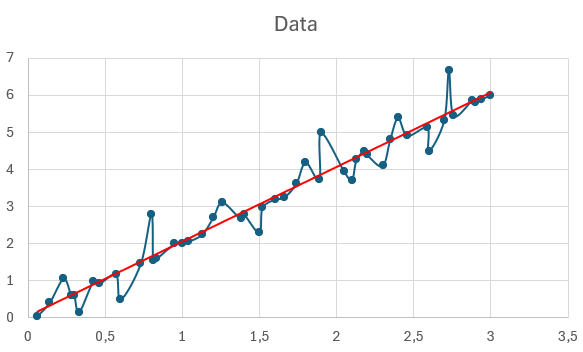
\includegraphics[width=0.8\textwidth]{static/overfitting.png}
    \caption{The blue line represents a model which is not well generalized, and thus captures the noise in the data.
    The red line represents a model which is well generalized, and thus captures the general distribution of the data.}
    \label{fig:overfitting}
\end{figure}

A model can also be designed to directly predict the aleatoric uncertainty, as a second output, in addition to the main prediction.
This requires a modification of the loss function to account for the uncertainty output.
How this is done in practice will be discussed in \cref{ch:models-for-uncertainty-aware-object-detection_section:training-evaluation}.

\subsection{Epistemic uncertainty} \label{ch:literature-study_section:quantifying-uncertainty_subsection:epistemic-uncertainty}
Quantifying epistemic uncertainty is more complex, as it requires evaluating multiple models, hyperparameters, and usage of data.
There are different methods to account for this uncertainty, especially in theory.

First, a Bayesian approach can be used to model parameter uncertainty (see \cref{ch:literature-study_section:uncertainty-aware-ai-models_subsection:bayesian-neural-networks}).
This is a very principled and theoretical way to model the uncertainty, as it requires an infinite ensemble of models to fully capture parameter uncertainty, which is not possible in practice.

An alternative approach utilizes an ensemble of \gls{dnn} (see \cref{ch:literature-study_section:uncertainty-aware-ai-models_subsection:deep-ensemble-methods}).
This is a more practical approximation of the Bayesian approach, using a finite number of models to estimate epistemic uncertainty.

A third method models uncertainty by keeping dropout active during inference (see \cref{ch:literature-study_section:uncertainty-aware-ai-models_subsection:monte-carlo-dropout}).
\gls{mc} dropout, like the ensemble method, is more practical than the Bayesian approach. 
By leaving dropout enabled during inference, the network generates multiple different outputs for the same input, which are then combined to calculate a final prediction and an associated uncertainty score.

\section{Uncertainty-aware AI models} \label{ch:literature-study_section:uncertainty-aware-ai-models}
Conventional \gls{ai} architectures, such as \glspl{mlp}, \glspl{cnn}, \glspl{gan}, and YOLO networks, are not inherently designed to quantify predictive uncertainty.
Consequently, new methodologies had to be developed to make these models uncertainty-aware.
The methods discussed below are rooted in Bayesian principles, offering a mathematically sound framework for modeling uncertainty.

\subsection{Bayesian Neural Networks} \label{ch:literature-study_section:uncertainty-aware-ai-models_subsection:bayesian-neural-networks}
A \gls{nn} is a function mapping an input $x \in X$ to an output $y \in Y$ via a model $f_{\theta}$, as shown in \cref{eq:nn}.
\begin{equation}
    y = f_{\theta}(x)
    \label{eq:nn}
\end{equation}
In our specific use case, the input vector $x$ is an image, and the output vector $y$ represents the predicted center coordinates of an object.
The model's parameters, $\theta$, are optimized during the training phase using a dataset of input-output pairs.

\paragraph{Aleatoric uncertainty}\cite{src:scalable-bayesian-deep-learning}
For standard regression problems, models typically predict target values directly using \cref{eq:nn}.
The parameters $\theta$ are learned by minimizing a loss function, such as $L^1$ or $L^2$ loss, over the training data.
However, this deterministic approach fails to capture aleatoric uncertainty, as it outputs a single value per target without any confidence metric.
Instead of predicting a discrete scalar, the model can be restructured to predict a probability distribution over the targets, as shown in \cref{eq:prob-dist}.
Assuming a Gaussian distribution, the network can predict both the mean $\mu$ and the variance $\sigma^2$, structured as in \cref{eq:nn-aleatoric-vec}.

\begin{subequations}
\label{eq:nn-aleatoric}
    \begin{align}
        p(y|x, \theta) &= \mathcal{N}(y; \mu_{\theta}(x), \sigma^2_{\theta}(x)), \label{eq:prob-dist} \\
        f_\theta(x) &= [\mu_{\theta}(x), \log\sigma^2_{\theta}(x)]^T \label{eq:nn-aleatoric-vec}
    \end{align}
\end{subequations}

Here, the variance $\sigma^2$ represents the aleatoric data uncertainty, while the mean $\mu$ serves as the core prediction.
This model is trained by minimizing the negative log-likelihood of the data relative to the predicted distribution, defined in \cref{eq:nn-aleatoric-loss}.
\begin{equation}
    min(-\sum_{i} \log(p(y_i|x_i, \theta)))
    \label{eq:nn-aleatoric-loss}
\end{equation}

\paragraph{Epistemic uncertainty}\cite{src:scalable-bayesian-deep-learning}\cite{src:bayesian-deep-learning-epistemic}
Capturing uncertainty in the model parameters $\theta$ requires a Bayesian approach, commonly known as Bayesian inference.
This method assigns a prior distribution to the model parameters, representing foundational beliefs before any data is observed.
By leveraging the training data, we compute a posterior distribution over $\theta$ (\cref{eq:posterior-distr}), representing updated parameter beliefs post-observation.

\begin{equation}
    p(\theta|X, Y) = \frac{p(Y|X, \theta)p(\theta)}{p(Y|X)}
    \label{eq:posterior-distr}
\end{equation}

The term $p(\theta)$ denotes the prior distribution over the parameters, chosen based on initial assumptions.
When no prior beliefs exist, a Gaussian distribution is most commonly applied.
However, the selection of this prior acts as a critical regularization mechanism~\cite{src:lecture-notes-bayesian-learning}:

\begin{itemize}
    \item $L^2$ regularization is equivalent to using a Gaussian prior.
    \item $L^1$ regularization is equivalent to using a Laplace prior.
\end{itemize}

The likelihood of the data given the parameters, $p(Y|X, \theta)$, measures how effectively the model fits the training observations.
This is calculated by processing the dataset through the model and determining the probability of the data under the resulting output distribution.
The evidence, $p(Y|X)$, acts as a normalizing constant to ensure the posterior forms a valid probability distribution.
It is determined by integrating the likelihood across all possible parameter values, as shown in \cref{eq:evidence}.

\begin{equation}
    p(Y|X) = \int p(Y|X, \theta)p(\theta)d\theta
    \label{eq:evidence}
\end{equation}

However, calculating this evidence analytically is practically impossible due to the massive parameter space typical of a \gls{dnn}.
Consequently, computing the exact posterior distribution is equally infeasible.
Therefore, robust approximations are necessary to estimate the posterior distribution effectively.

\subsection{Deep Ensemble Methods} \label{ch:literature-study_section:uncertainty-aware-ai-models_subsection:deep-ensemble-methods}
A deep ensemble method~\cite{src:deep-ensemble-methods} is based on the principle that a combination of models often outperforms a single, highly complex architecture.
Crucially, this approach naturally generates highly reliable uncertainty metrics alongside its predictions.
Unlike traditional ensembles that aggregate decision trees, deep ensembles utilize multiple independent \glspl{nn}.
Creating a deep ensemble requires three foundational components:
\begin{itemize}
    \item A proper scoring rule, which is used as a way to train the models in the ensemble.
    \item Adversarial training, which is used to make the models in the ensemble more robust.
    \item The actual ensembling, which combines the outputs of the different models to create a final output and uncertainty score.
\end{itemize}

\paragraph{The scoring rule}
A scoring rule mathematically measures the quality of a model's probabilistic outputs.
It must encourage the network to produce accurate classifications while heavily penalizing overconfident, incorrect predictions.
For example, if a model falsely predicts the presence of an object with absolute certainty, the scoring rule should inflict a severe loss penalty.
Conversely, it should reward the model for outputting lower, distributed probabilities when dealing with ambiguous visual inputs.
This calibration ensures the model is rightfully confident on clear data and appropriately hesitant on unknown or noisy data.
Fortunately, standard classification loss functions, such as softmax cross-entropy, inherently function as proper scoring rules.

\paragraph{Adversarial training}
Adversarial training is employed to increase model robustness against minute input perturbations that drastically alter outputs.
Usually, these changes are imperceptible to humans, yet they easily trick the network into making entirely false predictions.
For instance, an image confidently classified as a disk might be misclassified as a cube following an invisible alteration of a few pixel values.
Such erratic behavior must be prevented, as these massive swings in confidence destroy the reliability of the model's uncertainty metrics.
Adversarial training addresses this by generating synthetic training samples featuring these exact, minor perturbations.
The system generates adversarial images designed to fool the network, then feeds them back into the training loop with their true, correct labels.
Consequently, the model learns to ignore these tiny adversarial shifts, significantly stabilizing its output confidence.

\paragraph{Ensembling}
The final step in this methodology is the aggregation of the individual networks.
Research suggests deploying an ensemble of identical deep \glspl{nn} to simultaneously predict a target and an uncertainty score~\cite{src:deep-ensemble-methods}.
Each member of the ensemble trains independently, though they utilize the exact same underlying architecture.
By simply initializing the weights randomly and shuffling the training data batches independently, sufficient model variance is naturally achieved.
This eliminates the need for complex diversification techniques like bagging or boosting.
Consequently, the entire dataset can be utilized to train every model, which is highly beneficial for data-hungry deep learning architectures.
To generate the final prediction and uncertainty metric, the individual outputs are aggregated.
Each independent model outputs a probability distribution across the available classes.
These separate distributions are then averaged to form a singular, finalized output distribution.
The class possessing the highest averaged probability becomes the final prediction, with the variance acting as the uncertainty score.
We continue with the disk and cube classification example to illustrate this.
Assuming an ensemble of three models, they might output the following distributions for a given image:
\begin{itemize}
    \item Model 1: [0.7 (disk), 0.3 (cube)]
    \item Model 2: [0.4 (disk), 0.6 (cube)]
    \item Model 3: [0.9 (disk), 0.1 (cube)]
\end{itemize}
Averaging these arrays yields the final aggregated distribution: [0.67 (disk), 0.33 (cube)].
Thus, the final classification is 'disk' with an aggregated confidence score of 0.67.

\subsection{Monte Carlo dropout} \label{ch:literature-study_section:uncertainty-aware-ai-models_subsection:monte-carlo-dropout}
Dropout is a standard regularization technique utilized during \gls{nn} training to mitigate overfitting.
The core concept involves randomly deactivating a subset of neurons during each training pass.
This forces the network to distribute learned representations across all nodes rather than relying heavily on specific neural pathways.
Once training is complete, dropout is traditionally disabled for inference, utilizing the entire network for deterministic predictions.
\gls{mc} dropout expands upon this by intentionally leaving the dropout layers active during inference~\cite{src:mc-dropout}.
Each time a forward pass drops a random set of neurons, the functional architecture shifts slightly, resulting in variable outputs for the exact same input.
Each of these stochastic forward passes acts functionally similarly to an independent model within a deep ensemble.
By executing multiple forward passes with dropout enabled, the system generates a spread of distinct probability distributions for a single target.
These outputs are subsequently aggregated—much like the deep ensemble approach described in \cref{ch:literature-study_section:uncertainty-aware-ai-models_subsection:deep-ensemble-methods}—to derive a final prediction and an explicit uncertainty metric.
Returning to the disk and cube classification scenario, executing three forward passes using \gls{mc} dropout might produce the following:
\begin{itemize}
    \item Forward pass 1: [0.8 (disk), 0.2 (cube)]
    \item Forward pass 2: [0.5 (disk), 0.5 (cube)]
    \item Forward pass 3: [0.6 (disk), 0.4 (cube)]
\end{itemize}
Averaging these individual passes results in a final output distribution of [0.63 (disk), 0.37 (cube)].
The final prediction resolves to 'disk' with an aggregated confidence score of 0.63.